
\newcommand{\FigFragmentSingle}{
\begin{figure}
    \centering
    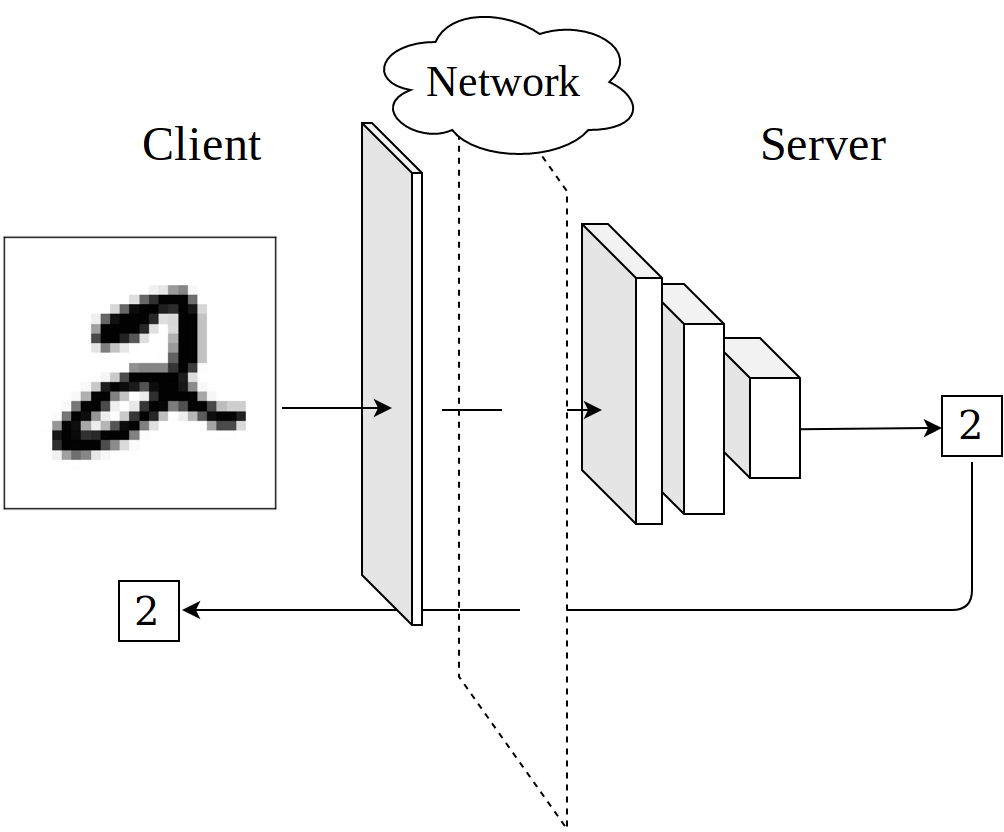
\includegraphics[width=0.4\textwidth]{images/diff_shard_nn-proposed.png}
    \caption{\textbf{Fragmented Machine}\,---\,%
        We propose fragmenting models into two pieces one of which will 
        be distributed to clients. In this way we can rely on the compression
        to latent manifolds to create privacy preserving classification services
        where the service doesn't learn the exact input.}  
    \label{fig:frag-single}
\end{figure}
}


\newcommand{\FigFragmentMany}{
\begin{figure}[t]
    \centering
    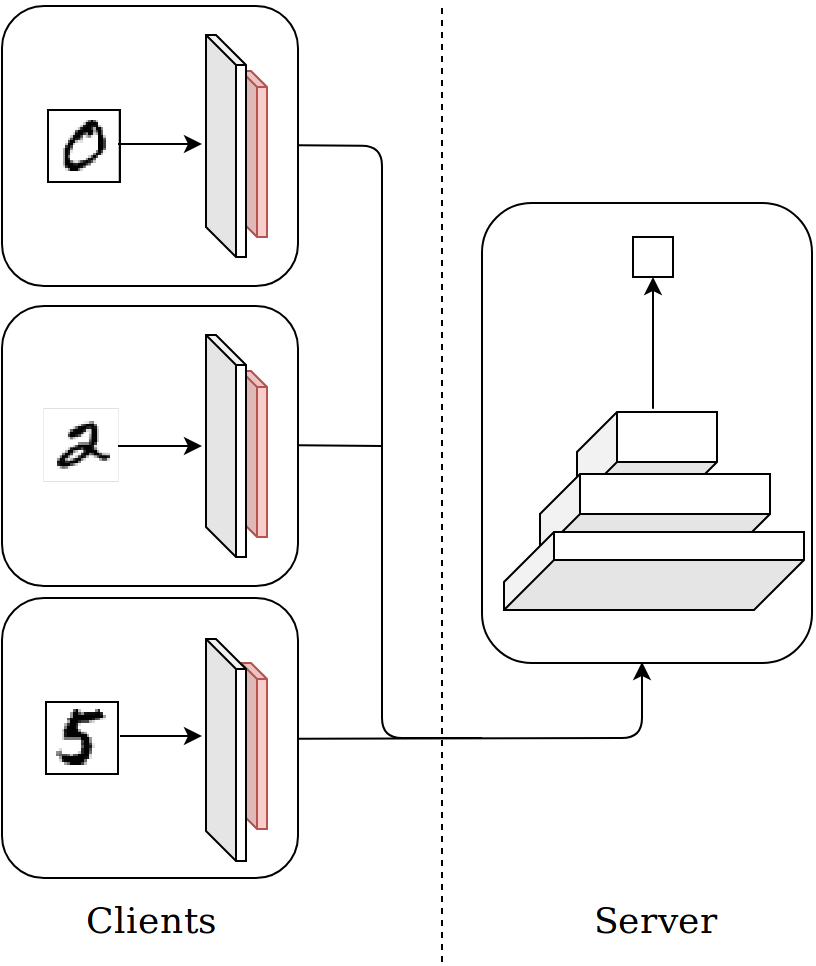
\includegraphics[width=0.4\textwidth]{images/diff_frag_many.png}
    \caption{\textbf{Multi-Party Machine}\,---\,%
        For a service that accommodates many users a fragmented model can distribute
        semi-unique portions of the model to each user. Each client then employs 
        techniques to increase the cost of inverting the model such that a service
        never truly operated on un-encoded data, and translating the data back to it's
        original domain is extremely (approximating prohibitively) expensive.}  
    \label{fig:frag-many}
\end{figure}
}
